\documentclass[11pt,a4paper,openany]{book}
\usepackage[utf8]{inputenc}
\usepackage[T1]{fontenc}
\usepackage{lipsum}  %juste utile ici pour générer du faux texte}
\usepackage{amsmath,amsfonts,amssymb} %extensions de l'ams pour les mathématiques
%\usepackage{tikz}
\usepackage{graphicx} %pour insérer images et pdf entre autres
\usepackage[left=2.5cm,right=2.5cm,top=1.5cm,bottom=2cm]
{geometry} %réglages des marges du document selon vos préférences ou celles de votre établissement
\usepackage{shorttoc} % Pour un sommaire simplifié en début du mémoire
\usepackage{fancyhdr} %pour les en-têtes et pieds de pages
\setlength{ \headheight}{14.2pt} % hauteur de l'en-tête
%%%%%%%%%%%%%%%%%%%style front%%%%%%%%%%%%%%%%%%%%%%%%%%%%%%%%%%%%%%%%%
 \fancypagestyle{front}{ %
 \fancyhf{} %on vide l'en-tête
 \renewcommand{\headrulewidth}{0pt} %trait horizontal pour l'en-tête
 \renewcommand{\footrulewidth}{0.4pt} %trait horizontal pour le pied de page
 }
%\renewcommand{\chaptermark}[1]{%
%\markboth{\MakeUppercase{%
%\chaptername}\ \thechapter.%
%\ #1}{}}
%%%%%%%%%%%%%%%%%%%style main%%%%%%%%%%%%%%%%%%%%%%%%%%%%%%%%%%%%
 \fancypagestyle{plain}{ %
		\fancyhf{}
		\renewcommand{\chaptermark}[1]{\markboth{\chaptername\ \thechapter.\ ##1}{}} % redéfinition pour avoir ici les titres %des chapitres des sections en minuscules
		\renewcommand{\sectionmark}[1]{\markright{\thesection\ ##1}}
	 \fancyhead[C]{}
	 \fancyhead[L]{\rightmark} %
	 \fancyhead[R]{\leftmark}
	 %\fancyfoot[C]{}
	 \fancyfoot[R]{page \thepage} %
	%\fancyfoot[RO,LE]{page \thepage} %
	 %\fancyfoot[LO,RE]{Mon rapport}
	\fancyfoot[L]{Mémoire de Master II rédigé par Tedjou Jospin} %
}
%%%%%%%%%%%%%%%%%%%style back%%%%%%%%%%%%%%%%%%%%%%%%%%%%%%%%%%%%%%%%%
 \fancypagestyle{back}{ %
 \fancyhf{} %on vide l'en-tête
 \fancyfoot[C]{page \thepage} %
 \renewcommand{\headrulewidth}{0pt} %trait horizontal pour l'en-tête
 \renewcommand{\footrulewidth}{0.4pt} %trait horizontal pour le pied de pages
 }


\usepackage[english, french]{babel} %pour un document en français
\usepackage{listings} %pour insérer du code source
\usepackage{hyperref} %rend actif les liens, références croisées, toc…
\hypersetup{colorlinks, %
 citecolor=black, %
 filecolor=black, %
 linkcolor=black, %
 urlcolor=black}

%%%%%%%%%%%%%%%%%%%%%%%%%%%%biblio%%%%%%%%%%%%%%%%%%%%%%%%%%%%%%%%%%%%%
\usepackage[backend=biber]{biblatex}
%\bibliography{plain}
\addbibresource{../bibliographie/bibliographie.bib} % pour indiquer où se trouve notre .bib
\usepackage{csquotes} % pour la gestion des guillemets français.

%%%%%%%%%%%%%%%%%%%%%%%%%%%%%glossaire%%%%%%%%%%%%%%%%%%%%%%%%%%%%%%%%%%%
\usepackage{glossaries}
\makeglossaries

%%%%%%%%%%%%%%%%%%%%%%%%%%%%%index%%%%%%%%%%%%%%%%%%%%%%%%%%%%%%%%%%%
\usepackage{makeidx}
\makeindex

%%%%%%%%%%%%%%%%%%%%%%%%%%%%liste des abréviations%%%%%%%%%%%%%%
\usepackage{nomencl}
\makenomenclature
\renewcommand{\nomname}{Liste des abréviations, des sigles et des symboles}

%%%%%%%%%%%%%%%% environnement pour les résumés%%%%%%%%%%%%%%%%%%%%\makeatletter
\newenvironment{abstract}{ %
 \cleardoublepage
 %\null\vfil
 %\@beginparpenalty\@lowpenalty
 \begin{center} %
		\bfseries \abstractname
		%\@endparpenalty\@M
 \end{center}} %
 {\par\vfil\null}
\makeatother



\begin{document}
%\frontmatter % début des pages liminaires
\pagestyle{front} %style des en-têtes pour cette partie
\begin{titlepage}
\parindent=0pt
 \hspace*{ \stretch{1}}  université de yaoundé 1
département d'informatique\hspace*{ \stretch{1}} 
\vspace*{ \stretch{1}}
\begin{center}
% \includegraphics[scale=0.5]{images/logo.png} %
\end{center}
\vspace*{ \stretch{1}}
\hrulefill
\begin{center} \bfseries\Huge
Spécification  formelle de l'architecture d'un éditeur de composants métiers caractéristiques
\end{center}
\hrulefill
\vspace*{1cm}
\begin{center} \bfseries\Large
Mémoire présenté en vue de l'obtention du diplome de MASTER II en informatique
\end{center}
\begin{center}\bfseries\Large
par Tedjou jospin delmas
\end{center}
\begin{center} \bfseries\Large
Sous la direction de Dr. Amougou Ngoumou.
\end{center}
\vspace*{ \stretch{2}}
\begin{flushright}
 Le \today
\end{flushright}

\end{titlepage}

\cleardoublepage
%\input{page_de_couverture/page_de_titre}
%\thispagestyle{empty} % pour une page sans en-tête ni pieds de page
%\chapter*{Résumés}
\addcontentsline{toc}{chapter}{Résumé} %Pour l'ajout dans la table des matières au même rang que chapitre
\begin{abstract}
Mon résumé: Les lignes de produit logiciel...Les lignes de produit logiciel...Les lignes de produit logiciel...Les lignes 
\end{abstract}
\thispagestyle{empty} %idem pour la page blanche qui suit
\selectlanguage{english} % pour un typographie anglaise
\renewcommand{\abstractname}{Abstract} %pour changer le titre
\begin{abstract}
My abstract: Software prodcut lines.....Software prodcut lines.....Software prodcut lines.....Software prodcut 
\end{abstract}
\thispagestyle{empty} %
\selectlanguage{french} % on n'oublie pas de repasser en langue française. %no comment !
%\vspace*{ \stretch{1}}
\begin{flushright}
\` Amon père, ma mère, mes frères zé mes sœurs, oho...
\end{flushright}
%\vspace*{ \stretch{2}} %no comment !
%\shorttableofcontents{Sommaire}{0} %sommaire avec uniquement les chapitres
\tableofcontents %table des matières plus complète
\addcontentsline{toc}{chapter}{Table des matières} %ajout de la table des matières dans la table des matières !
%\addcontentsline{toc}{chapter}{Sommaire} %ajout du sommaire dans le sommaire !

%\mainmatter % corps du document
%\pagestyle{main} % style des en-têtes pour cette partie
\chapter{Introduction}
\addcontentsline{toc}{chapter}{Introduction}
\markboth{Introduction}{}

\section*{contexte}
De nos jours, il n'est plus possible d'imaginer un secteur d'activité qui ne fait pas usage des outils logiciels. On les utilise  dans le domaine de la finance, des transports, la gestion de stocks, l'éducation et bien d'autres. Leur mise en place est toutefois très coûteuse en termes de budget, d’effort, de temps de réalisation et sujette à des risques d’échec. Il devient alors intéressant de produire des logiciels de meilleure qualité à faible coût et rapidement; c'est le but principal de l'ingénierie de ligne de produits logiciels \cite{Klaus2005}.  Elle se base sur le fait que les logiciels développés aujourd'hui ne sont pas nouveaux mais sont des variantes de systèmes déjà développés dans le même secteur d’activité \cite{Fouda2009}. Dans le domaine de la gestion académique par exemple, un système logiciel pour une nouvelle université est une variante des systèmes existants, déployés dans les autres universités et qui a ses propres spécificités. Il traitera comme les autres des étudiants, des enseignants, des matières, des notes mais peut avoir son propre système de notes différent de celui des autres logiciels du domaine. Un domaine peut être vu comme \glsdesc{domaine} \cite{Klaus2005}.

Au lieu de construire des logiciels en partant de rien (from scratch), l'objectif désormais est de construire des familles de logiciels desquelles seront dérivés les logiciels du domaine. Les connaissances accumulées dans le domaine concerné sont ainsi exploitées. 
Comme le souligne Urli \cite{Urli2015}, plusieurs définitions sont utilisées dans la littérature pour qualifier les Lignes de produits mais celle de Clements et Northrop est très souvent citée dans les travaux du domaine. Selon elle, une famille de logiciels ou ligne de produit logiciel (LPL) est \glsdesc{LPL_def} \cite{Clements2002}. 

\section*{problématique} 
Le développement des lignes de produits se fait par une nouvelle idéologie appelée Ingénierie de ligne de produits logiciels qui vise la production des familles de logiciels ou lignes de produits logiciels. Pohl et al. définissent l’ingénierie des LPL comme \glsdesc{ILP_def} \cite{Klaus2005}. 

L'ingénierie de ligne de produits est constituée de deux étapes principales: l'ingénierie de domaine et l'ingénierie applicative \cite{Klaus2005}. L'ingénierie de domaine analyse le domaine pour en cerner les propriétés communes aux applications du domaine (commonalities en anglais) et les propriétés variables (variabilities en anglais) afin de produire l'ensemble des artéfacts logiciels réutilisables. L'ingénierie applicative quant à elle permet de construire les logiciels membres de la famille selon les besoins spécifiques en utilisant les artéfacts produits par l'ingénierie de domaine en exploitant la variabilité. Ainsi, le développement d'un nouveau  logiciel revient à analyser les besoins spécifiques, paramétrer la plateforme support en choisissant les composants adéquats et générer le code du logiciel. L'ingénierie de ligne de produit fait alors intervenir l'Ingénierie Dirigée par les Modèles(IDM) lors de la dérivation d'un produit de la ligne \cite{Ngassam2017}.

Plusieurs méthodes de développement de lignes de produits ont été proposées dans la littérature: FAST(Family oriented Abstraction, Specification and Translation), PuLSE (Product Line Software Engineering)  ,ODM (Organization Domain Modeling), DARE (Domain Analysis and Reuse Environment), FODA (Feature Oriented Domain Analysis), FORM(Feature Oriented Reuse Method) etc. La méthode FORM étend la méthode FODA basée sur les caractéristiques (features) qui a été longuement exploitée dans les applications industrielles. 

En 2009, le Professeur \emph{Marcel FOUDA NDJODO} et le Docteur \emph{AMOUGOU NGOUMOU} ont proposé la méthode FORM/BCS (Feature Oriented Reuse Method with Business Component Semantics) \cite{Fouda2009} qui étend la méthode FORM pour entre autre élargir son application aux systèmes d’information. C'est cette méthode qui suscite notre intérêt dans le cadre de ce travail.

\section*{question de recherche et résultats attendus}
La méthode FORM/BCS ne dispose pas encore d’outils support pour permettre son exploitation dans la pratique. La question principale qui motive ce travail est alors la suivante. Comment peut se présenter la description formelle d'un éditeur de composants métiers caractéristiques? Cette question est d'autant plus importante que les composants métiers caractéristiques sont au centre de FOMR/BCS, il est donc indispensable de fournir aux ingénieurs logiciel un éditeur basé sur ladite méthode qui facilite la saisie des composants métiers caractéristiques.   Dès lors dans le cadre de ce travail, nous voulons contribuer à la mise en place d’une plateforme support pour la manipulation dynamique des lignes de produits de FORM/BCS. Nous nous attellerons plus spécifiquement à la conception et à l’implémentation de l’architecture d’un éditeur de composants métiers caractéristiques (\textit{feature business components}) en tant que plug-in Eclipse à l’aide de l’outil EMF (Eclipse Modeling Framework). 

\section*{méthodologie}
Pour réaliser ce travail, nous devons tout d'abord comprendre la méthode FORM/BCS en étudiant les propriétés du modèle, puis étudier l'embryon de plate-forme support actuelle de FORM/BCS ainsi que le plugin EMF (Eclipse Modeling Framework) et ses dérivés. Enfin il nous reviendra de donner une description formelle de l'éditeur de composants métier caractéristiques de FORM/BCS pour permettre l'expansion de la plateforme.

\section*{plan}
Ce travail est structuré comme suit. D'abord le chapitre 1 présente l'état de l'art des architectures de quelques outils de ligne de produits logiciels. Ensuite le chapitre 2 explique la méthode FORM/BCS en détaillant les caractéristiques du modèle de FORM/BCS. Puis, le chapitre 3 présente la mise en œuvre qu'il nous a été donné de réaliser, il récapitule les étapes de réalisation de l'éditeur de composant métier caractéristique de FORM/BCS et décrit l’architecture de ce dernier. 




\chapter{Revue de la littérature}
Nous présentons dans ce chapitre un état de l’art des méthodes d'ingénierie de ligne de produits. Dans un premier temps, nous parcourrons les concepts de l'ingénierie de ligne de produits acceptés des chercheurs du domaine. Ensuite nous présentons quelques plateformes existantes de l'ingénierie de ligne de produits. 

\section{Ingénierie de lignes de produits}
En réponse à la difficulté de produire des logiciels de qualité à moindre coût et en respectant les délais, les industries et les universités se sont penchées, autour des années 2000, vers une nouvelle idéologie consistant à produire des familles de logiciels plutôt que des logiciels indépendants: c'est l'ingénierie de ligne de produits logiciels. L’idée derrière les LPL est de maximiser la production de logiciels présentant des similarités, issus d’une même famille de produits, par la réutilisation systématique d’une même base de code et par la définition de variantes \cite{Urli2015}. 

Clements et al. \cite{Clements2002} définissent une famille de logiciels ou ligne de produits logiciels (LPL) comme \glsdesc{LPL_def}. Cette définition fait ressortir le fait que les logiciels d'une famille sont développés à partir du même ensemble d’artefacts logiciels et repondent chacun à un besoin spécifique bien que provenant d'une base commune de code. L’ingénierie de ligne de produits ne vise donc pas à produire des logiciels pour satisfaire un besoin isolé comme traditionnellement, elle vise plutôt la satisfaction d'une large gamme de besoins dans un secteur d'activité ou domaine donné. Chaque logiciel de la famille répondant à un besoin particulier de ce domaine et ayant des points communs avec les autres logiciels de sa famille et ses propres spécificités qui le différencient des autres, communément nommées variantes. Elle tire avantage de la réutilisation de code et la personnalisation de masse. Le domaine est d'abord minutieusement étudié, une fois la ligne de produit construite, le développement d'un logiciel membre se fait par configuration de la plate-forme support et la réutilisation de composants pour répondre aux besoins spécifiques.

Le processus de développement des lignes de produits se fait en deux étapes, l'ingénierie du domaine et l'ingénierie de l'application. Le produit final étant une architecture qui servira de socle au développement des produits du domaine et des composants réutilisables qui seront exploités lors de la production des logiciels de la famille. La figure \ref{fig:framework_ILP} ci-dessous présente le Framework de l'ingénierie de ligne de produits.

\begin{figure}[h!]
  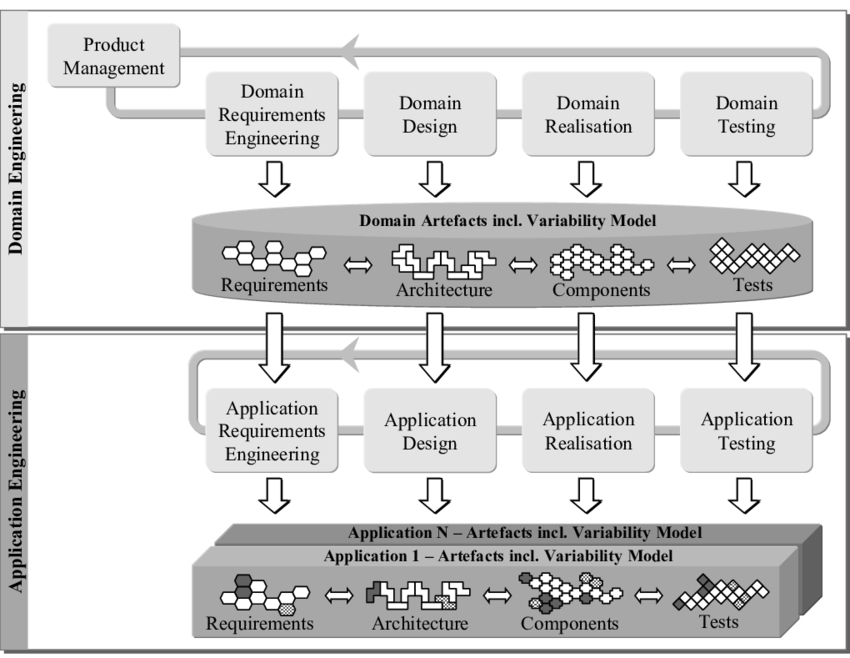
\includegraphics[scale=0.9999, width=150mm]{images/SPLE_Framework.png}
  \caption{framework de l'ingénierie de ligne de produits}
  \label{fig:framework_ILP}
\end{figure}

\subsection{Ingénierie de domaine}
Le développement d'une ligne de produits logiciels nécessite une bonne compréhension du domaine concerné et une fluide expression de la variabilité, qui est l'ensemble des propriétés qui diffèrent d'une application à une autre. Un domaine peut être vu comme \glsdesc{domaine} \cite{Klaus2005}. L'ingénierie de domaine est alors \glsdesc{ingenierie_de_domaine} \cite{Klaus2005}. Elle se réalise en trois phases:
\begin{itemize}
	\item \textbf{l'analyse du domaine} qui est l'activité qui décrit et représente formellement les concepts de base du domaine ainsi que la variabilité. Avant de faire une analyse du domaine, il faut au préalable définir les frontières du domaine à analyser. Elle vise à réaliser un modèle du domaine qui spécifie formellement les informations de celui-ci. Une bonne analyse de domaine se mène en plusieurs activités: la définirion du dictionnaire des termes du domaine, la documentation des hypothèses du domaine, l'identification des acteurs du domaine, l'identification des problèmes du domaine, l'identification des artéfacts existants et l'identification de la similarité et de la variabilité.
	\item \textbf{la spécification de l’infrastructure}, Elle prend en entrée le modèle produit à l'étape précédente et décrit l’organisation des artefacts réutilisables (spécifications, diagrammes, code etc.),
	\item \textbf{l’implémentation de l'infrastructure} qui comprend l’implémentation des artefacts définis à l'étape précédente
\end{itemize}  
\subsection{Ingénierie de l’application}
Elle permet de developper les nouvelles applications du domaine à partir de la plate-forme et des composants réutilisables créés aucours de l'ingénierie de domaine. La réalisation du produit durant l’ingénierie de l’application est généralement automatisée à partir des choix effectués au sein de la représentation abstraite définie lors de l’ingénierie du domaine \cite{Awais2011}. La production des produits logiciels se fait par la configuration de la plateforme et la réalisation du produit qui est souvent automatisée. Cette derniere activité fait intervenir des techniques avancées de l'ingénierie logicielle telles que l’ingénierie dirigée par les modèles et la programmation générative \cite{Urli2015}. L'ingénierie de l'application suit un cycle de vie <<classique>> où chaque étape est facilitée par les artéfacts de l'ingénierie de domaine.
\begin{itemize}
	\item \textbf{Analyse des besoins} La définition des besoins.
	\item \textbf{Conception de l'application} La spécification de la solution permettant de satisfaire ces
besoins.
	\item \textbf{Implémentation} L’implémentation de cette solution.
	\item \textbf{Tests et validation} La phase de test de la solution et son évaluation par
rapport aux besoins initiaux.
\end{itemize}
\subsection{Introduction à la variabilité}
Les applications d'une LPL ont certes beaucoup de points communs mais aussi des différences que l'on exprime par la notion de variabilité. La variabilité peut être définie comme \glsdesc{variabilite} \cite{Hugo2013}. Pour maîtriser cette variabilité, il faut distinguer "le sujet de la variabilité" (ce qui varie), de "l'objet de la variabilité" (comment cela varie) et du "point de variiation" (comment la variabilité se réalise au sein de la ligne). Pol et al. \cite{Klaus2005} résument cela en trois questions:

\begin{itemize}
	\item  Qu'est ce qui varie ?
	\item Pourquoi est-ce-que cela varie ?
	\item Comment cela varie-t-il ?
\end{itemize}
Les assertions suivantes font ressortir des propriétés qui varient: 

\begin{itemize}
	\item  Une voiture peut avoir un toit fixe ou ouvrant.
	\item Une personne a des enfants qui peuvent être des garçons ou des filles.
	\item Un ordinateur peut être équipé d’une deuxième batterie ou d’un lecteur de DVD.
\end{itemize}
Il est donc question d'intégrer la variabilité dans les artefacts réutilisables dès l'analyse du domaine et dans toutes les autres phases (elle est intégrée dans le modèle du domaine, les spécifications, l'architecture, les composants, les scénarios de test etc. \cite{Magnus2003}). Le but étant d’accroître la flexibilité de la plate-forme et des composants. Lorsque cela est bien fait, la dérivation d'un produit membre se fait essentiellement par la sélection des bons artefacts et la génération du code source.
\subsection{Modélisation de la variabilité}
Dans la littérature, plusieurs approches ont été proposées pour modéliser la variabilité. Une des plus acceptées est la méthode \textbf{FODA} \glsdesc{FODA} basée sur les \textsl{features} proposée par Kang et al. en 1990. Un feature ou caractéristique métier est \glsdesc{feature} \cite{Kyo1990}. La méthode FODA distingue trois types de caractéristiques métiers:

\begin{itemize}
	\item  Les caractéristiques obligatoires, qui sont communes à tous les produits de la ligne.
	\item Les caractéristiques optionnelles, qui sont facultatives.
	\item Les caractéristiques alternatives. C'est un petit ensemble dont on ne peut choisir qu'un élément à un moment donné.
\end{itemize}

\section{Les plateformes de Lignes de produits}
\subsection{FAMA}
FAMA(FeAture Model Analyser) \cite{Benavodes2007} est un Framework d’analyse automatique des Feature Models dans les LPL. En effet, la gestion des grands Features Models avait déjà été décrite dans la littérature comme une tâche difficile et sujette à des erreurs. Ces Features Models contiennent des informations très utiles comme par exemple le nombre de produits potentiel modélisés, les features du noyau de la plateforme et les features variants de la ligne de produit. FAMA se propose alors d'analyser automatiquement les features models et d'en extraire les informations utiles et détecter des éventuelles erreurs. Le modèle théorique de FAMA est basé sur les Features Models étendus avec des cardinalités sur lesquels on applique la programmation par contraintes. Un exemple de CSP(Constraint Satisfaction Problem) est donné par l'illustration suivante.
\begin{figure}[h!]
  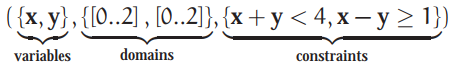
\includegraphics[scale=0.9999, width=150mm]{images/exemple_constraint_satisfaction_problem.PNG}
  \caption{Exemple de problème satisfaisant une contrainte \cite{Benavodes2007}}
  \label{fig:FORM_Process}
\end{figure}

L'analyse d'un Feature Model se fait en deux étapes: il est d'abord traduit en une représentation logique puis des solveurs procèdent à l'extraction des informations. Un prototype nommé FAMA-EP a été développé en tant que plug-in Eclipse. Il offre deux principales fonctionnalités: la création et la modification visuelle de modèles et l'analyse automatique de ces modèles. Une fois que l'utilisateur crée ou importe un Feature Model, l'analyse peut commencer. FAMA-EP intègre plusieurs solveurs pour l'analyse pour plus d'efficacité. Il permet entre autre de déterminer si un feature model est non vide (s'il peut produire au moins un produit), trouver le nombre total de produits, lister tous les produits possibles du Feature Model, calculer l'ensemble de features communs. 
L'architecture de ce plug-in se constitue d'un éditeur visuel et d'un moteur d'analyse qui se charge de trouver le meilleur solveurs pour effectuer l'analyse demandée sur le Feature Model. Nous notons que FAMA est éfficace pour l'analyse des Features Models puisqu'il utilise plusieurs solveurs cependant il ne couvre pas toutes les étapes de l'ingénierie de ligne de produit.
 
\subsection{PURE::VARIANTS}
PURE::VARIANTS \cite{PureVariants} est une plateforme professionnelle, livrée comme plug-in Eclipse ou standalone application pour supporter le développement et le déploiement des lignes de produits logiciels. La ligne de produits logiciels est ici décrite en trois parties principales; Feature Models, Family Models et Variant Description Model. \textbf{Le Feature Model} décrit les produits de la ligne en terme de features qui sont communs à ces produits et de features qui varient d'un produit à un autre ainsi que les relations entre ces features; un feature étant une propriété d'un produit qui sera visible par l'utilisateur du produit. \textbf{Le Family Model} quant à lui décrit comment les produits de la ligne seront assemblés ou générés à partir des composants existants; chaque composant représente un ou plusieurs éléments fonctionnels des produits de la ligne (classes, objets, variables etc.). Chaque élément du Family Model a des contraintes qui spécifient s'il doit être inclus, par défaut tout élément dont le parent est inclus est également inclus. \textbf{Le Variant Description Model} (VDM) décrit l'ensemble des features d'un produit de la ligne. C'est dans ce modèle que l'on indique les features à choisir parmi ceux du Feature Model pour un produit spécifique à générer. PURE::VARIANTS offre un editeur pour spécifier et valider les features pour la configuration d'un produit (\textit{VDM editor}). Plusieurs versions de PURE::VARIANTS sont en vente en ligne parmi lesquelles PURE::VARIANTS for AUTOSAR pour la création et la maintenance des modèles réutilisables AUTOSAR, PURE::VARAINTS for IBM Rationnal Doors pour la gestion de la varaibilité dans les besoins fonctionnels des applications, PURE::VARAINTS for Enterprise architect pour la création et la maintenance des modèles UML et SysML.
 
\subsection{FeatureIDE}
FeatureIDE \cite{hum2012} est un framework gratuit basé sur Eclipse qui supporte les étapes du développement de logiciel basé sur les features. Il supporte plusieurs techniques d'implémentation des logiciels à partir des features telles que la programmation orientée feature, la programmation par aspects, la programmation orientée Delta et  les préprocesseurs. Le but principal de cet outil est de couvrir le cycle complet de développement et d'incorporer les outils dans des environnements de développement intégré (EDI). Son architecture facilite le développement d'outils supports pour les langages existants et les nouveaux langages pour les lignes de produits. FeatureIDE est beaucoup plus un outil pour la recherche et l'enseignement. Il est utilisé à Austin (au Texas), Magdebourg (en Allemagne), Marbourg (en Allemagne), Santa Cruz (en Californie), Turin (en Italie). Cet outils pourvoit un éditeur graphique de features Models qui permet de construire des features models en ajoutant et en enlevant des features. Cet éditeur permet de déplacer un feature (avec ses sous-features) sur un nouveau feature parent. FeatureIDE en lui même se concentre sur l'analyse du domaine; pour couvrir le cycle complet de l'ingénierie de ligne de produit, des extensions doivent être ajoutée au framework pour supporter l'implémentation du domaine et la génération de logiciel. Plusieurs extensions implémentant diverses approches sont disponibles. AHEAD, FeatureHouse, FeatureCpp, DeltaJ, AspectJ, Munge en sont quelques unes.  
       
\subsection{SPLOT}
SPLOT(Software Product Line Online Tool) \cite{Marcilio2009} est un système web développé en java qui utilise un générateur de template HTML pour créer des environnements hautement interactifs avec des interfaces utilisateurs de raisonnement et de configuration basées sur Ajax(Asynchronious Javascript And XML). Puisqu'il est basé sur internet, il facilite grandement le partage de connaissance notamment à travers le dépôt de features models et ne nécessite pas de téléchargement de mises à jour . Il offre deux principaux services: le raisonnement automatisé et la configuration du produit. Le raisonnement est axé sur l’automatisation du calcul statistique (profondeur de l'arbre de features, nombre de features etc.) et le débogage critique (cohérence des features models, détection des features morts etc.). Disponible en ligne à l'adresse \textsl{http://splot-research.org}, SPLOT a un riche dépôt de features models contenant près de 20 modèles réels précedement publiés dans la litterature et plusieurs modèles générés. L'éditeur graphique de feature de SPLOT permet de modifier un des modèles existants ou d'en créer un nouveau. Il permet d'ajouter un nouveau feature obligatoire, optionnel ou un groupe de features alternatifs. L'ajout des règles entre features dans SPLOT se fait en ajoutant des règles sous la forme de conjonction de littéraux dans laquelle les littéraux sont des features ou leur négation. A titre d'exemple pour signifier que l'inclusion d'un feature A oblige l'inclusion d'un feature B, la règle s'écrit comme suit: 
\lnot$FeatureA  \lor$ FeatureB. Pour rendre ette proposition vraie, le Feature A et le Feature B doivent être sélectionnés mais elle est également vraie quand le Feature B est choisi et pas Feature A. 

\subsection{Points de comparaison entre ces outils}
Nous dressons ci-dessus un tableau comparatif des outils de ligne de produits précédemment décrits. Les critères arrétés pour cette analyse sont les suivants:
 
 \begin{itemize}
	 \item  La portée: qui définit si le logiciel est open source ou à but commercial
	 \item  Le langage utilisé pour développer l'outil
	 \item  L’existence d'un éditeur de features intégré dans l'outil
	 \item  l'existance d'une description formelle de l'éditeur visuel qui permet de bien comprendre l'architecture interne de l'éditeur et l'étendre au besoin.
 \end{itemize}

\begin{table}[b]
\begin{tabular}{|l|c|c|c|r|}
  \hline
  \textbf{Outils} & \textbf{Portée} & \textbf{Langage} & \textbf{Editeur intégré} & \textbf{Description formelle} \\
	\hline
  \textsl{FAMA} & open source & Java & oui & non \\
  \hline
  \textsl{PURE::VARIANTS} & commerciale & Java & oui & non \\
	\hline
  \textsl{FeatureIDE} & open source & Java & oui & non \\
	\hline
  \textsl{SPLOT} & open source & Java & oui & non \\
	\hline
  \textbf{REAL} & \textbf{open source} & \textbf{Java} & \textbf{oui} & \textbf{oui} \\
  \hline
\end{tabular}
\caption{Tableau comparatifs des outils de LPL\label{time}} 
\end{table}

Nous faisons la remarque selon laquelle le langage Java et la plateforme Eclipse sont très utilisés pour le développement d'éditeurs de features mais ces derniers manquent le plus souvent de description formelle. Pourtant une bonne description formelle des éditeurs faciliteraient la compréhension des outils par les tierces et l'extensibilité. Notre travail pour la suite sera alors de décrire de façon formelle l'architecture de l'éditeur de la méthode FORM/BCS nommé REAL.


\chapter{Méthode Formelle de description des architectures logiciel}
L'architecture des systèmes logiciel est très souvent décrite de façon informelle sous forme de diagrammes composés de boîtes et de lignes les reliant \cite{Gregory1995}. Cependant, bien que ces diagrammes soient interprétés en suivant des conventions définies, la nature informelle et imprécise de ses interprétations a de nombreuses limites. Nous pouvons citer à titre d'exemple l'ambiguïté dans la compréhension des architectures, la difficulté à analyser et tester automatiquement les modèles. 
\section{Description du langage  Z}
Développé à l'universite d'Oxford, le langage Z \cite{Gregory1995} est un langage formel. Ses racines mathématiques reposent essentiellement sur la logique de premeir ordre et la théorie des ensembles. La notation de Z utilise les connecteurs logiques standard (\land$, \lor$, \lnot, =>, etc.) et les opérations sur les ensembles (\in$, \cup$, \cap$, \subset$, etc.) tout en gardant leur signification originale. Pour décrire un système, les types (ou ensembles donnés) qui seront utilisés dans la spécification sont généralement listés au départ.

\subsection{Schéma de Z}
Dans la notation Z, les spécifications sont représentées par des boites compartimentées appelées \textit{schémas}. Un schéma décrit l'état d'un système ou les opérations possibles sur ce dernier. Un exemple de schéma est donné ci-après, il décrit l'enregistrement des passagers dans un avion. On considère pour cet exemple le type [PERSONNE] qui est l'ensemble des personnes identifiées de façon unique.

\begin{schema}{Avion}
capacite: \nat; aBord: \power_1~PERSONNE
\where
#aBord <= capacite
\znewpage
\end{schema}

La première partie de notre schéma contient les définitions de deux variables: capacité et aBord qui représentent respectivement la capacité de l'avion et le nombre de personnes à bord. La deuxième partie contient les contraintes sur ces variables. Dans notre cas, le nombre de personnes à bord de l'avion ne doit pas excéder la capacité de l'avion, ce qui est logique. 

\section{Formalisation d'une architecture de composants}
Pour représenter les architectures de logiciels à un niveau très abstrait, les composants sont souvent utilisés. Ces derniers interagissent entre eux pour faire fonctionner le système entier. Nous allons dans la suite nous intéresser à la formalisation d'une architecture de composants en utilisant \textbf{la notation Z}. Nous utiliserons pour se faire les travaux de \texttt{GREGORY D. ABOWD et al} dans \cite{Gregory1995}. 

Les trois éléments de base d'une architecture de composants sont: les composants, les connecteurs et les configurations des composants et connecteurs. 
\subsection{Les composants}
Les composants sont des unités fonctionnelles actives d'un système (voir figure \ref{fig:Z_component}). Ils accomplissent des tâches en faisant des traitements internes et des communications externes avec le reste du système. L'interaction entre les composants est définie explicitement comme une collection de points d'interaction ou ports. De façon intuitive, le port généralise la notion traditionnelle d'interface de modules. Dans les cas simples, un port peut représenter une procédure qui peut être appelée ou une variable qui peut être accédée dans l'interaction avec un autre composant. Un port peut tout aussi bien représenter, dans les cas plus complexes, une collection de procédures, un ensemble d’événements. Un composant, vu comme entité syntaxique, est un ensemble constitué de ports et d'une description de son traitement.
\begin{figure}[h!]
  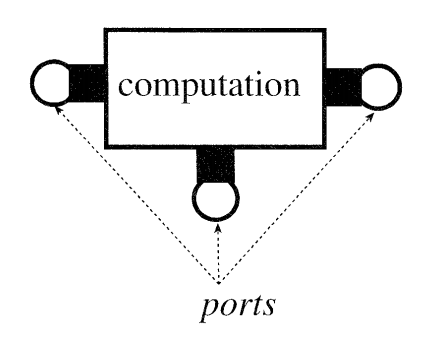
\includegraphics[scale=0.7]{images/composant_Z.png}
  \caption{Un composant}
  \label{fig:Z_component}
\end{figure}
La représentation formelle d'un composant avec la notation Z est donnée par la figure \ref{fig:Z_component_schema}.
\begin{figure}[h!]
  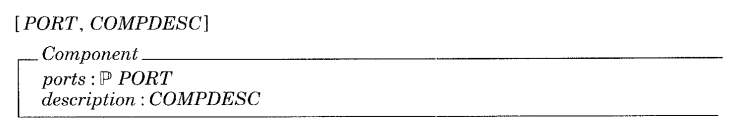
\includegraphics[scale=0.7]{images/Z_component_schema.png}
  \caption{Représentation d'un composant}
  \label{fig:Z_component_schema}
\end{figure}

\subsection{Les connecteurs}
Les connecteurs définissent les interactions entre composants (voir figure \ref{fig:Z_connector}). Ils permettent à des composants d'interagir en définissant la façon, le protocole de cette interaction. Tout comme les composants, les connecteurs sont des entités indépendantes. Un connecteur a une interface qui consiste en un ensemble de rôles. Chaque rôle définit le comportement que l'un des participants de l'interaction doit avoir. A titre d'exemple, un connecteur client-serveur a un rôle demandeur (le client) et un rôle fournisseur (le serveur); de même, un connecteur multicast aura un rôle annonceur et plusieurs rôles receveurs. Le comportement global d'un connecteur et des règles qu'il spécifie est défini de façon logique par un protocole. Par exemple, le protocole d'un connecteur client-serveur, nécessite que l'initialisation se fasse avant l'envoie de toute requête. Un connecteur architectural est alors modélisé comme une collection constituée de rôles et de la description de son protocole d'interaction comme décrit dans le schéma Connector.
\begin{figure}[h!]
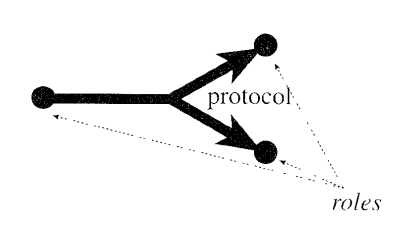
\includegraphics[scale=0.7]{images/connecteur_Z.png}
  \caption{Un connecteur}
  \label{fig:Z_connector}
\end{figure}
La représentation formelle d'un connecteur avec la notation Z est donnée par la figure \ref{fig:Z_connector_schema} suivante.
\begin{figure}[h!]
  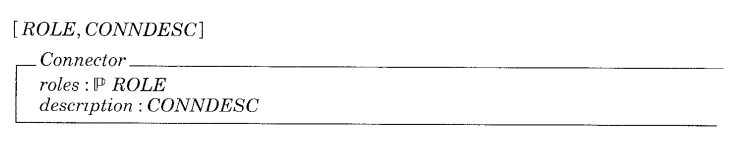
\includegraphics[scale=0.7]{images/Z_connector_schema.png}
  \caption{Représentation d'un connecteur}
  \label{fig:Z_connector_schema}
\end{figure}

\subsection{Les configurations}
Une configuration est une collection d'instances de composants qui interagissent au moyen d’instances de connecteurs (voir figure  \ref{fig:Z_configuration}). Les instances de composants et de connecteurs sont identifiés en nommant les éléments à partir de la classe syntaxique. Pour nommer les instances de composants et de connecteurs, nous introduisons deux ensembles: COMPNAME des noms possibles de composants et CONNNAME des noms de connecteurs. Ces ensembles sont aussi utilisés pour nommer les instances de ports associés à un composant ou de rôles associés à un connecteur.   Ainsi nous introduisons deux nouveaux types PortInst de tous les ports disponibles et RoleInst des instances de rôle illustré par la figure \ref{fig:Z_portInst_roleInst}.
\begin{figure}[h!]
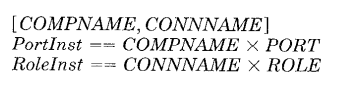
\includegraphics[scale=0.7, width=100mm]{images/Z_portInst_roleInst.png}
  \caption{PortInst et RoleInst}
  \label{fig:Z_portInst_roleInst}
\end{figure}

L'association entre les instances de composants et de connecteurs est modélisée par \texttt{des attachements} entre les rôles des connecteurs et les ports des composants.
\begin{figure}[h!]
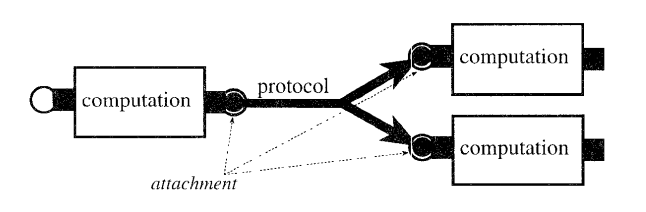
\includegraphics[scale=0.7]{images/configuration_Z.png}
  \caption{Une configuration}
  \label{fig:Z_configuration}
\end{figure}
La représentation formelle d'un connecteur avec la notation Z est donnée par la figure \ref{fig:Z_configuration_schema}.
\begin{figure}[h!]
  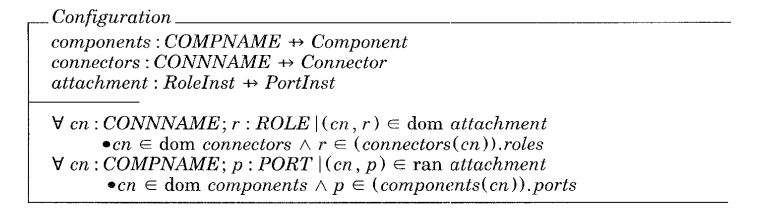
\includegraphics[scale=0.7]{images/Z_configuration_schema.png}
  \caption{Représentation d'une configuration}
  \label{fig:Z_configuration_schema}
\end{figure}

Le schéma \textsl{configuration} impose deux contraintes additionnelles (en dessous de la ligne de séparation) qui seront satisfaites par toutes les configurations. La première spécifie que toute instance de rôle dans l'attachement est un rôle pour un connecteur nommé dans la configuration. La seconde contrainte quant à elle assure que toutes les instances de ports décrites par la configuration doivent apparaître dans une instance actuelle de composants. Ces deux contraintes font respecter une portée lexicale sur les attachements au sein d'une configuration.

\chapter {Description formelle de l'éditeur de composants métiers caractéristiques}

\section{Présentation de l'éditeur}
L'embryon de plateforme existant pour la méthode FORM/BCS a été développé en Java en utilisant le framework Eclipse EMF(Eclipse Modeling Framework). EMF est un environnement de modélisation et de génération de code qui facilite la construction d'outils et d'applications sur les modèles de données structurées. Il est basé sur l'Ingénierie Dirigée par les Modèles (IDM); l'approche de développement IDM consiste à séparer les spécifications fonctionnelles d'un système de son implémentation. Elle préconise pour ce faire de construire trois principaux modèles pour aboutir à la génération du code source 
\begin{itemize}
	\item CIM (Computational Independent Model) qui modélise les exigences fonctionnelles du système
	\item PIM (Platform Independent Model) ou encore modèle conceptuel qui est un modèle abstrait, indépendant de toute plateforme d'exécution 
	\item PSM (Platform Specific Model) qui est un modèle technologique de plus bas niveau dépendant de la plateforme d'exécution.
	\item Le code source est généré à partir de la PSM. 
	\end{itemize}
	
	La figure figure \ref{fig:MDA_process}
	
\begin{figure}[h!]
  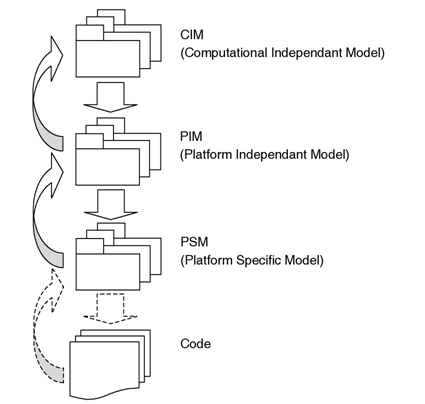
\includegraphics[scale=0.7]{images/mda_technology.png}
  \caption{Processus de Ingénierie Dirigée par les Modèles}
  \label{fig:MDA_process}
\end{figure}
	
	Ainsi, EMF génère du code source en transformant différents modèles. Il permet également de générer des éditeurs textuels ou graphique. Le point d'entrée est un modèle appelé Ecore, c'est le Méta-modèle d'EMF, il est indépendant de la plateforme d'execution car ne contient aucne information à propos des packages ou des classes Java. Ce dernier peut être spécifié en utilisant l'éditeur graphique qu'offre EMF ou en important des interfaces Java, un diagramme de classe UML ou un schéma XML. Le méta-modèle Ecore étant indépendant de toute plateforme d'exécution, pour générer du code Java, il faut spécifier un modèle de génération qui contient les informations de plateforme (packages, classes...): c'est le \textsl{genmodel}; il peut être généré automatiquement à partir du modèle Ecore. Associé à EMF, le plugin EMFTEXT permet de générer des éditeurs pour les DSL (Domain Specific Language) avec des fonctionnalités avancées telles que l'autocomplétion, la coloration du texte, la personnalisation de la syntaxe, le rapport instantané des erreurs etc. C'est ce plugin qui a été utilisé pour la réalisation de l'embryon de plateforme pour le projet REAL. 

\begin{figure}[h!]
  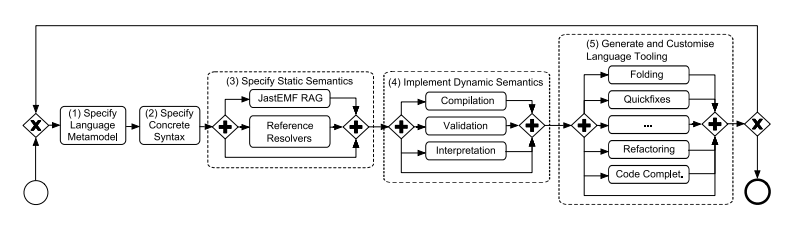
\includegraphics[scale=0.7]{images/EMFTEXT_process.png}
  \caption{Processus de développement d'un langage avec EMFTEXT}
  \label{fig:EMFTEXT_process}
\end{figure}

La génération d'un éditeur sophistiqué pour un nouveau langage necessite juste quelques étapes de spécification et de génération avec EMFTEXT comme le montre la figure \ref{fig:EMFTEXT_process}. Ces étapes sont les suivantes:
\begin{enumerate}
	\item spécifier le métamodèle Ecore
	\item spécifier la syntaxe concrète
	\item (optionnelle) spécifier la sémantique statique 
	\item (optionnelle) implémenter la sémantique dynamique 
	\item générer et (optionnellement) modifier l'éditeur, par exemple en personnalisant la complétion de code, la mise en valeur de la syntaxe etc.
\end{enumerate}

De ces étapes, seules les étapes (1) et (2) sont obligatoires ainsi que la génération du code de l'éditeur (étape 5). C'est par ces dernières que le plugin REAL a été généré. 
\subsection{Description non-formelle de l'embryon}
Le plugin généré a été baptisé REAL. Il se compose des différents éléments suivants:
\begin{enumerate}
	\item spécifier le métamodèle Ecore
	\item spécifier la syntaxe concrète
	\item (optionnelle) spécifier la sémantique statique 
	\item (optionnelle) implémenter la sémantique dynamique 
	\item générer et (optionnellement) modifier l'éditeur, par exemple en personnalisant la complétion de code, la mise en valeur de la syntaxe etc.
\end{enumerate}
\begin{figure}[h!]
  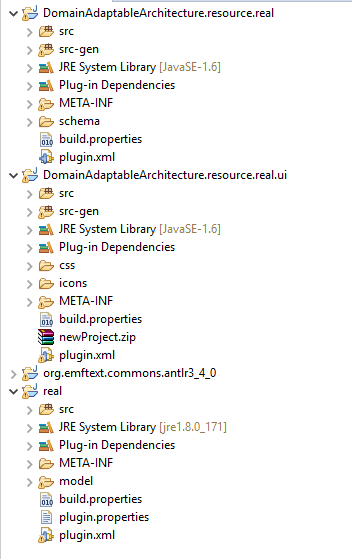
\includegraphics[scale=0.9]{images/real.png}
  \caption{Plugin REAL}
  \label{fig:plugin_real}
\end{figure}
\section{Description formelle}
1.Décrire les packages de REAL sous forme de composants(modules)
2.Montrer la communication entre ces modules
3.Parler des EXTENSIONS POINTS


\chapter*{Conclusion}
\addcontentsline{toc}{chapter}{Conclusion}
\markboth{Conclusion}{}

\cleardoublepage % le corps du document est terminé
\appendix
%\pagestyle{back}
%\input{annexes/annexe1}
%\input{annexes/annexe2}
%\backmatter
\thispagestyle{empty}
\chapter*{Remerciements}
\addcontentsline{toc}{chapter}{Remerciements}
Merci à Namrod pour toute la partie sur la bibliographie. Retrouvez ses questions FAQ qui ont permis larédaction de cette
%\noindent Merci à f-leb, LittleWhite et Metalman pour leurs conseils et la relecture.
%\noindent Merci à ced et jacques pour la correction orthographique et typographique.
 %no comment !

\newacronym{LPL}{LPL}{Ligne de produit logiciels}
\newacronym{ILP}{ILP}{Ingénierie de Ligne de Produits}
\newacronym{EMF}{EMF}{Eclipse Modeling Framework}
\newacronym{FODA}{FODA}{Feature Oriented Domain Analysis}
\newacronym{FORM}{FORM}{Feature Oriented Reused Method}
\newacronym{DSL}{DSL}{Domain Specific Language}

\newglossaryentry{LPL_def}
{
        name={LPL},
        description={un ensemble de logiciels partageant des propriétés communes, satisfaisant des besoins spécifiques pour un domaine donné et développés de façon contrôlée à partir d'un ensemble commun d’artefacts}
}
\newglossaryentry{domaine}
{
        name={domaine},
        description={un secteur d'activité ou une zone de connaissance dirigé par un ensemble de besoins et caractérisé par des concepts et des terminologies compréhensibles par les acteurs de ce secteur}
}
\newglossaryentry{ILP_def}
{
        name={ILP},
        description={un paradigme de développement de logiciels utilisant une plateforme logicielle commune et la personnalisation de masse}
}
\newglossaryentry{ingenierie_de_domaine}
{
        name={ingénierie},
        description={le processus de l'ingénierie de ligne de produits qui permet l'analyse, la spécification et l'implémentation des artéfacts logiciels dans un domaine qui sont utilisés pour construire les systèmes logiciels dans ce domaine}
}
\newglossaryentry{variabilite}
{
        name={variabilité},
        description={l'ensemble des différences, décrites de façon structuré, de toutes ou d'une partie des caractéristiques d'une famille de logiciels}
}
\newglossaryentry{feature}
{
        name={caractéristique},
        description={un aspect, une qualité ou une caractéristique, d'un logiciel ou d'une famille de logiciel, importante et visible par l'utilisateur}
}
\printglossaries
\addcontentsline{toc}{chapter}{Glossaire}
\printnomenclature
\addcontentsline{toc}{chapter}{Liste des abréviations, des sigles et des symboles}
\nocite{*}
\printbibliography
\addcontentsline{toc}{chapter}{Bibliographie}
\listoffigures
\addcontentsline{toc}{chapter}{Table des figures}
\listoftables
\addcontentsline{toc}{chapter}{Liste des tableaux}
\end{document}
